\subsection{Satteins}
Das Testgebiet von "'Fast and Curious"' war in der Gemeinde Satteins. Diese Gemeinde liegt östlich von Feldkirch im Bundesland Vorarlberg in Österreich. Da Herr Prof. Dr. Klaus Frick in dieser Ortschaft in der Gemeindevertretung tätig ist, wurde eine Bewilligung zur Aufstellung der Geräte ausgehändigt. Dort konnten die Geräte installiert und für mehrere Tage in Betrieb gehalten werden. In den folgenden Punkten wird das Gebiet beschrieben und anschliessend darauf eingegangen, wie die Daten erfasst wurden.

\subsubsection{Topologie}
Im nachfolgenen Bild (\fref{bSatteins}) ist die Topologie von Satteins dargestellt. In dieser Darstellung sind die Aufstellpunkte der sechs Geräte mit einem schwarzen Punkt schematisch markiert. Jedes dieser Geräte wurde an den Ein- und Ausfahrtspunkten, sowie an strategisch interessanten Verkehrspunkten platziert. Dadurch sollte eine möglichst effiziente Auswertung durchgeführt werden können. Somit ist es mit diesen sechs Geräten möglich, den grössten Teil des Verkehrsflusses in der besagten Ortschaft quantitativ rekonstruieren zu können. 

\begin{figure}[H]
  \centering
  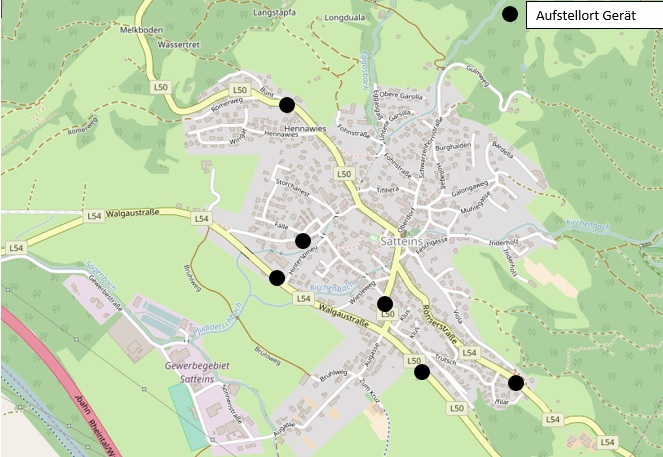
\includegraphics[width=0.99\textwidth]{Resultate/Satteins.jpg} 
  \caption{Topologie von Satteins. \cite{satteins}}
  \label{bSatteins}
\end{figure}
\newpage
Mit der Hilfe des folgenden Bildes (\fref{bGraph}) wurden die wichtigsten Abzweigung, welche die Verkehrsteilnehmer nehmen können, identifiziert und in der Berechnung des Verkehrsflusses beachtet. Durch den Graphen konnten auch die wichtigsten Punkte ermittelt werden, wo die Geräte aufgestellt werden sollten, um eine möglichst effiziente Verfolgung garantieren zu können. Bei diesem Verkehrsnetz beinhaltet dies, die vier wichtigen Zufahrtsstrassen zum Gebiet und ebenfalls zwei relevanten Strassen innerhalb. Daraus lässt sich der Verkehrsfluss im Graphen darstellen und im Anschluss auf die Karte von Satteins zurück projizieren.

\begin{figure}[H]
  \centering
  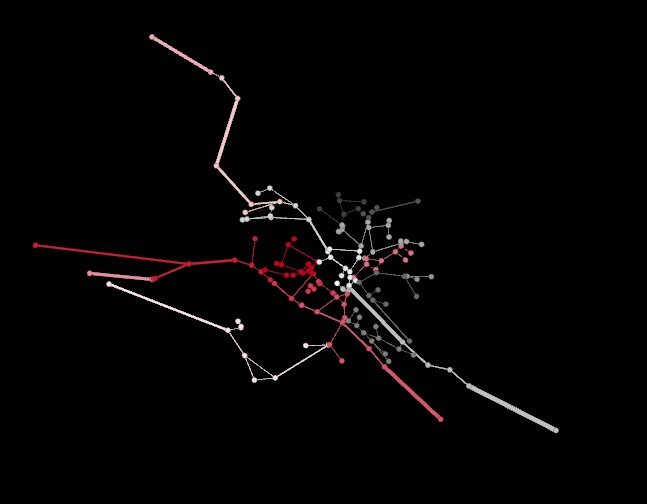
\includegraphics[width=0.99\textwidth]{Resultate/Topologie.jpg} 
  \caption{Graph des Verkehrsnetzes von Satteins.}
  \label{bGraph}
\end{figure}

\subsubsection{Erfassung der Daten}
Alle Daten, welche die Geräte aufgezeichnet haben, wurden auf den internen SD-Karten abgespeichert und jeden zweiten Tag mittels Smartphone-Hotspot auf den Laptop übertragen. Dabei wurde bei jedem einzelnen Gerät der Feature Vektor, sowie der Temperaturverlauf heruntergeladen. Die Feature Vektoren der Geräte enthielten mehrere tausend Einträge mit vorbeigefahrenen Verkehrsteilnehmern.